\section{Recommender system}\label{Recommender-system}
It would be beneficial to provide a way for users to see relevant, interesting services for their preferences, in order to make the system more usable.
To accomplish this, a recommender system can be used.
The following section will detail different ways of implementing such a system, which one we chose and why, and finally our implementation of a recommender system.

\subsection{The purpose of a recommender system}
When searching for something new, information overload can occur.
Many different sources can provide information that might not be relevant.
If a new user interacts with this system, seeking to find a new subject in which to attain knowledge, this user could potentially be presented with an overwhelming amount of services, depending on how many tutors have made these available.
Another issue that might arise is that not all of the services will be relevant for the new user, serving only to clog the list of services. 
This leads to information overload, where the retrieved information in the form of services is not what the user needs, and not enough of the correctly relevant information is returned.
Recommender systems are used to remedy these issues.
They help match users with relevant items, in this case services, to ease the information overload.
This generates value for both the user and the tutor, in that users are matched with what they have a predilection for, and tutors can reach more prospective students.
We discuss two methods of creating a recommender, \textit{content-based filtering} and \textit{collaborative filtering}.

\subsection{Content-based filtering}\label{content-based-filtering}
Content-based recommender systems recommend an item to a user based upon a description of the item and a profile of the user's interests \cite{ContentBasedFiltering}.
A common scenario for web applications is that they present a list of items to a user, and the user then selects among these to receive more details. 
An item in such a scenario would have a representation dependent on the implementation, which could be used to analyze items of particular interest for a user.
Items are often stored in databases, creating structured data with each entry having the same set of attributes. 
This lends itself well to learning a user profile through different machine learning algorithms.
Examples of a basic representation of items and users are shown in Tables \ref{tbl:content-item} and \ref{tbl:content-user}.
As shown, users and items are represented by the same set of attributes.
\begin{table}[H]
    \centering
    \begin{tabular}{|l|l|l|l|l|}
    \hline
    Title                                         & Genre    & Author        & Price & Type      \\ \hline
    Blue Moon                                     & Thriller & Lee Child     & 10    & Hardcover \\ \hline
    Norse Mythology                               & Fantasy  & Neil Gaiman   & 6     & Paperback \\ \hline
    Normandy ‘44: D-Day and the Battle for France & History  & James Holland & 14    & Hardcover \\ \hline
    \end{tabular}
    \caption{This figure shows a possible representation of a few items for content-based filtering.}
    \label{tbl:content-item}
\end{table}
\begin{table}[H]
    \centering
    \begin{tabular}{|l|l|l|l|l|}
    \hline
    Title                                         & Genre    & Author        & Price & Type      \\ \hline
    ... & Fantasy  & George R. R. Martin, J.K. Rowling & 5    & Paperback \\\hline
    \end{tabular}
    \caption{This figure shows a possible representation of a user.}
    \label{tbl:content-user}
\end{table}
\noindent
The basic idea for content-based filtering is then to compute the similarity of an unseen item with the user profile, and suggest the items with attributes that are most similar to those in the user profile..
Unstructured data, such as text fields with no restriction, create complications when creating a user profile, as relationships between the values on an attribute for different items for a specific user can be found, but an unrestricted text will generally be unique \cite{ContentBasedFiltering}. 
If a user liked different restaurants based on the same cuisine, it could be indicated that this user would be likely to like other restaurants focused in the same cuisine as well, but a text review would not necessarily give this information.
Many domains can be represented by semi-structured data where issues arising from certain types of unstructured data, such as text fields, are converted to a structured representation \cite{ContentBasedFiltering}.
A user profile shows the preferences of the user, and consists mainly of two types of information:
\begin{itemize}
    \item A description of the types of items that interest the user
    \item A history of the user's interactions with the recommender system, such as storing the items that a user has viewed and information related to the interaction, such as if the user purchased the item.
\end{itemize}
Historical data of interactions can be used to filter out already purchased items, display recently visited items or as training data.
Creating a model of a user's preferences is then done through a form of classification learning, in which training data is divided into categories, an example being the binary categories \textit{Items the user likes} and \textit{items the user dislikes} \cite{ContentBasedFiltering}.
These algorithms learn a function that model's a users interests, and given a new item and the user model, this function predicts whether or not the user is interested in the item through a probability or a numeric value by analyzing the item representation and user profile.
Popular learning approaches for content-based filtering are \textit{naïve Bayes}, \textit{nearest neighbor methods} or \textit{linear classifiers}.

\subsection{Collaborative filtering}
Collaborative filtering differs from content-based filtering in that it focuses on matching users and items through the opinions of other people.
Collaborative filtering is based on word-of-mouth recommendations.
A person might have friends that recommend different things, and will eventually learn which of these friends has tastes that most align with their own, and thus which recommendation to value the most.
Collaborative filtering extends this concept \cite{CollaborativeFiltering}.
Collaborative filtering makes use of ratings.
These could be ratings between 1-5 or 1-10, for example, or simply binary ratings.
A rating is an association of two things, a user and a value.
A matrix of ratings can then be constructed, as shown in \autoref{tbl:collaborative-example}.
The empty entries indicate that the user has not rated the item, and are what the system should be able to predict.
\begin{table}[H]
    \centering
    \begin{tabular}{|l|l|l|l|l|}
    \hline
           & Item1 & Item2 & Item3 & Item4 \\ \hline
    Peter  & 3     &       & 5     &       \\ \hline
    Amy    & 4     & 2     &       & 3     \\ \hline
    Lars   &       & 5     & 3     & 2     \\ \hline
    Martin & 1     &       & 2     & 4     \\ \hline
    \end{tabular}
    \caption{This figure shows an example of a ratings matrix, with ratings from 1 to 5. An empty entry indicates that the user has not rated the item.}
    \label{tbl:collaborative-example}
\end{table}
\noindent
Domains with certain properties lend themselves to collaborative filtering. 
These are \textit{data distribution}, \textit{underlying meaning} and \textit{data persistence} \cite{CollaborativeFiltering}.
Data distribution encompasses domains in which there are many items, many ratings per item, more users rating that items to be recommended and users rate multiple items.
Underlying meaning encompasses domains in which users can have tastes in common, evaluation of an item cannot be done objectively and items are homogenous.
Data persistence encompasses domains in which items persist and taste persists, meaning the tastes of the users do not change rapidly.
Collaborative filtering usually makes use of \texttt{k nearest neighbor} algorithms based on users or items, or latent factor models to create predictions.
The user-based nearest neighbor approach focuses on finding users with similar tastes from which to predict a given user's rating, whereas the item-based approach focuses on finding items similar to a given item, and then taking the user's ratings for those similar items to predict a rating for an unrated item.
The latent factor approach focuses on splitting the rating matrix into separate matrices through matrix factorization to simulate communities, and creating predictions from these.


\subsection{Pros and cons}\label{sec:recommender-pros-and-cons}
Content-based filtering and collaborative filtering use different underlying assumptions \cite{CollaborativeFiltering}.
Content-based filtering assumes that items with similar objective features will be rated similarly, whereas collaborative filtering assumes that people with similar tastes rate things similarly, and that customers who had similar tastes in the past will have similar tastes in the future.
The assumption that collaborative filtering employs, that users will have similar taste in the future, is quite strong and cannot be guaranteed, as tastes are likely to change over time.
Content-based filtering can predict relevance for items without ratings by looking at similar items, whereas collaborative filtering requires ratings for an item to create predictions.
This means content-based filtering is especially useful for items that change a lot, but it needs content to analyze.
For domains where content is scarce, such as for a system in which users rate movies since a small amount of users will actually leave a rating, collaborative filtering has an edge since it does not require content.
Content-based techniques can have problems with new users, as there is a ramp-up phase when learning a model of the user's interests.
To do so, it needs explicit or implicit feedback, and there is no guarantee that the user leaves explicit feedback such as a rating, and implicit feedback from a user's behavior can be imprecise.
Since collaborative filtering requires ratings for an item to create predictions it has issues with cold starts.
If a new item is added, it will not have any initial ratings from users, which means creating a prediction becomes different as it has nothing from which to base the prediction.
Collaborative filtering methods making use of \texttt{k nearest neighbor} methods can have scalability issues, as the rating matrix can grow to be very large as more users join the service or more items are added.
This is a problem that latent factor models alleviate, as they reduce the size of the rating matrix through splits.
Content-based and collaborative filtering are not mutually exclusive, and both can be used in a complementary fashion to avoid some of the issues that arise when using just one.
\begin{table}[]
    \begin{tabular}{|p{.2\textwidth}|p{.4\textwidth}|p{.4\textwidth}|}
    \hline
                    & Content-based                                              & Collaborative                                                             \\ \hline
    Assumptions     & Items with similar features are rated similarly            & People with similar taste rate items similarly, taste will not change     \\ \hline
    Requirements    & Does not need ratings, but content to analyze              & Needs ratings but not content                                             \\ \hline
    Item changes    & Deals well with changing items by looking at similar items & Does not deal well with new items, as it needs initial ratings on an item \\ \hline
    Start-up issues & New users can have large ramp-up                           & Cold starts with new items                                                \\ \hline
    \end{tabular}
    \caption{A comparison of the pros and cons}
    \label{tab:recprosandcons}
    \end{table}

\subsection{Our choice}
Ideally, a combination of both collaborative and content-based filtering is ideal.
However, for this project implementing such a combination was not feasible, and we had to focus on one type of recommender system.
The reason it was not feasible was due to the recommender system being based on knowledge acquired from one of the semester courses, and such systems were only detailed towards the end of the semester, leading to a lack of time to create a combined solution.
The system has a simple rating system in which users rate a service on a numerical scale of one to five.
It is assumed that services will be rated by a small subset of users, since not all users will participate in all services, and not all who participate in a given service will leave a rating of it.
This means the domain will have content that is scarce.
It is also assumed that services will not change a lot.
If a service is based around swimming, we do not expect that it will quickly be changed to feature another subject matter, but rather a new service be added by the same tutor with the new subject matter.
As such, the better choice would be collaborative filtering, as the domain lends itself more to this type of system.
In terms of which approach to collaborative filtering to use, the added scalability of a latent factor model provides it an edge for this system as it focuses on scalability.

\subsection{Collaborative filtering through a latent factor model}
The latent factor model approach to collaborative filtering is an approach that tries to explain the ratings by characterizing both items and users on a number of factors.
This number of factors is usually 20-100 \cite{MatrixFactorization}. 
The factors are thought of as measures that measure dimensions.
For example, for movies, the factors could be thought of as measuring obvious dimensions such as amount of action, less well-defined dimensions such as character development or uninterpretable dimensions \cite{MatrixFactorization}.
\autoref{fig:latent-factor} shows an example of a latent factor approach with two dimensions.
It shows an example of how users and movies could be characterized based on the dimensions.
A user's predicted rating for a movie would then be equal to the dot product of the user's and movie's location on the graph, for example, user 5 would be expected to like movie 1, think movie 4 is average and dislike movie 2.
\begin{figure}[H]
    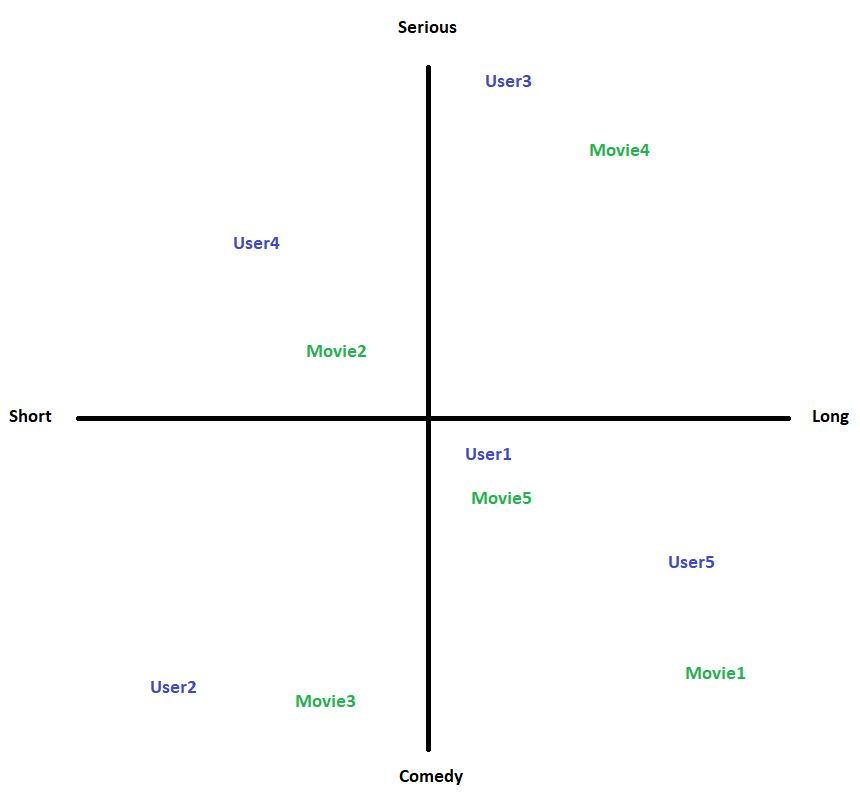
\includegraphics[width=\linewidth]{/recommender/latentfactor.JPG}
     \caption{A simplified illustration of a latent factor approach.}
     \label{fig:latent-factor}
 \end{figure}
 \noindent
A popular method of approaching a latent factor model is through matrix factorization.
Matrix factorization aims to characterize items and users by vectors of factors, and a recommendation would be found by a similarity between these.

\subsubsection{Matrix factorization}
Matrix factorization map users and items to a latent factor space of dimensionality \textit{f} \cite{MatrixFactorization}. 
This is achieved by taking the ratings matrix and splitting it into two matrices of the following dimensions, where $N_{i}$ is the number of items, $N_{u}$ is the number of users and $f$ is the number of factors:
\begin{equation}
    N_{i} \times f
\end{equation} 
\begin{equation}
    f \times N_{u}
\end{equation}
This results in each item \textit{i} and each user \textit{u} being associated with vectors: 
\begin{equation}
    q_{i} \epsilon \mathbb{R}^f
\end{equation}
\begin{equation}
    p_{u} \epsilon \mathbb{R}^f
\end{equation}
For a given item, the elements of $q_{i}$ measures the extent to which an item possesses the factors, and the elements of $p_{u}$ measures the interest of a user in items that are highly valued on the corresponding factor \cite{MatrixFactorization}.
The dot product of these two vectors then describes the user's overall interest in the item, leading to an estimate of:
\begin{figure}[H]
    \centering
    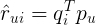
\includegraphics[]{/recommender/predictrating.png}
     \caption{How a prediction for a rating is calculated}
     \label{fig:predictrating}
 \end{figure}
 \noindent
To learn the factor vectors $p_{u}$ and $q_{i}$ used for the equation in \autoref{fig:predictrating}, the recommender system minimizes the squared error of the set of known ratings, that is, the entries in the ratings matrix that have a value:
 \begin{figure}[H]
    \centering
    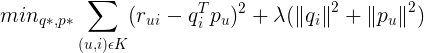
\includegraphics{/recommender/minimizesquarederror.png}
     \caption{How to calculate the squared error once predictions have been made}
     \label{fig:minimizesquarederror}
 \end{figure}
 \noindent
 In \autoref{fig:minimizesquarederror}, $K$ is the set of $(u, i)$ pairs for which the rating $r_{ui}$ is known.
 The system learns by fitting previously observed data, but to avoid overfitting when predicting future ratings, it regularizes the learned parameters.
 This regularization is found on the right side of the $+$ operator of the equation, where $\lambda$ is an arbitrary constant that controls the extent of the regularization.
 Stochastic gradient descent is one approach of minimizing the above equation.
 The algorithm will, in this approach, loop through all data in the training set, which is the known ratings.
 For each case, the system predicts a rating, and then computes the prediction error with the equation defined in \autoref{fig:calculatingerror}:
 \begin{figure}[H]
    \centering
    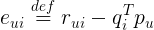
\includegraphics[]{/recommender/calculatingerror.png}
     \caption{The equation for calculating the error of a prediction when the actual value is known}
     \label{fig:calculatingerror}
 \end{figure}
 \noindent
 After the error has been calculated, the algorithm modifies the parameters through the updates rules shown in Figures \ref{fig:updatingq} and \ref{fig:updatingp}:
 \begin{figure}[H]
    \centering
    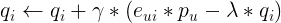
\includegraphics[]{/recommender/updatingq.png}
     \caption{The rule for updating the value of $q$}
     \label{fig:updatingq}
 \end{figure}
 \noindent
 
 \begin{figure}[H]
    \centering
    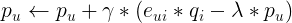
\includegraphics[]{/recommender/updatingp.png}
     \caption{The rule for updating the value of $p$}
     \label{fig:updatingp}
 \end{figure}
 \noindent
 For the update rules, $\gamma$ is the magnitude to which the parameters are modified, and is arbitrary.
 The calculations are performed until the squared error reaches a sufficiently small value, or a max number of iterations has been performed by the algorithm.
 
\subsection{Our implementation}
In \autoref{lst:recomstart} we initially make use of our other services to get the required data to predict ratings.
To perform the calculations we need all users, all services and all ratings currently in the database.
We then initialize the necessary matrices.
These are matrices with dimensions of respectively $users \times servcices$, $users \times factors$, $factors \times services$. 
For the ratings matrix which is $users \times services$ we call a function to populate it.
This is done by traversing the matrix, and for each rating in the \texttt{allRatings} variable, we search the ratings matrix for ids corresponding to the service and user ids of that rating.
If found, we insert the rating value into that entry.
\begin{lstlisting}[caption={The start of the recommender}, captionpos=b, label={lst:recomstart}]
export default class Recommender {
    static async calculateRecommendations(): Promise<number[][]> {
        const allUsers = await UserService.getAll();
        const allServices = await ServiceService.getAll();
        const allRatings = await RatingService.getAll();
    
        let userServiceMatrix: number[][] = [];
        let predictedRatings: number[][] = [];
        let userFactorMatrix: number[][] = [];
        let factorServiceMatrix: number[][] = [];

        userServiceMatrix = initUserServiceMatrix(numberOfRows, numberOfCols, allUsers, allServices, userServiceMatrix);

		userServiceMatrix = populateUserServiceMatrix(allRatings, numberOfRows, numberOfCols, userServiceMatrix);
(*@\centerline{\raisebox{-1pt}[0pt][0pt]{$\vdots$}}@*)
\end{lstlisting}
When we initialize both the matrix for users and factors as well as the matrix for factors and services we initialize all entries with random values between 0 and 1.
Initialization is illustrated in \autoref{lst:initUserFactor}.
This is done to ensure we can calculate a predicted rating.
The actual value is arbitrary, but a small value is chosen, as this should make the algorithm arrive at a model faster, compared to initializing with a greater value \cite{FunkMatrixFactorization}.
\begin{lstlisting}[caption={Initializing the user and factor matrix}, captionpos=b, label={lst:initUserFactor}]
function initUserFactorMatrix(numberOfRows: number, numberOfFactors: number, userFactorMatrix: number[][]): number[][] {
    for (let i = 0; i < numberOfRows; i++) {
        userFactorMatrix[i] = []; // Initialize inner array
        for (let j = 0; j < numberOfFactors; j++) {
            userFactorMatrix[i][j] = Math.random();
        }
    }   
    return userFactorMatrix;
}
\end{lstlisting}
\autoref{lst:initUserService} illustrates how we initialize the matrix for users and services.
On the first row we insert the ids of all services, and on the first column we insert all user ids.
This is done to ensure we can get the proper ids for the users and services to recommend.
Then we insert 0 in all entries, and call another function to populate the entries in which there are ratings.
If there is a rating from a user on a given service, we find the entry corresponding to these ids and insert the rating value.
This means we end with a matrix consisting of a row of service ids, a column of user ids, the rating values and 0 for those entries without ratings.
\begin{lstlisting}[caption={Initializing the user and service matrix}, captionpos=b, label={lst:initUserService}]
    export function initUserServiceMatrix(
	numberOfRows: number,
	numberOfCols: number,
	allUsers: User[],
	allServices: Service[],
	userServiceMatrix: number[][],
): number[][] {
	userServiceMatrix[0] = [];
	for (let i = 0; i < numberOfRows; i++) {
		userServiceMatrix[i + 1] = [];
		userServiceMatrix[i + 1][0] = allUsers[i].id;
	}

	for (let i = 0; i < numberOfCols; i++) {
		userServiceMatrix[0][i + 1] = allServices[i].id;
	}

	for (let i = 1; i < numberOfRows + 1; i++) {
		for (let j = 1; j < numberOfCols + 1; j++) {
			userServiceMatrix[i][j] = 0;
		}
	}

	return userServiceMatrix;
}
\end{lstlisting}
After initializing the matrices, we start the first calculation of predictions.
To do so, we call the function in \autoref{lst:dotmatrices} to calculate the dot products of the user by factor and factor by service matrices.
It simply iterates over a row from one matrix and a column for the other, multiplying the corresponding entries of each matrix, and adding them together.
The sum is then inserted into the predictedRatings matrix.
\begin{lstlisting}[caption={Calculating the dot predict of a matrix}, captionpos=b, label={lst:dotmatrices}]
function dotMatrices(
    numberOfRows: number,
    numberOfCols: number,
    numberOfFactors: number,
    userFactorMatrix: number[][],
    serviceFactorMatrix: number[][],
): number[][] {
    const predictedRatings: number[][] = [];
    let sum = 0;
    for (let i = 0; i < numberOfRows; i++) {
        predictedRatings[i] = [];
        for (let j = 0; j < numberOfCols; j++) {
            for (let k = 0; k < numberOfFactors; k++) {
                sum = sum + userFactorMatrix[i][k] * serviceFactorMatrix[k][j];
            }
            predictedRatings[i][j] = sum;
            sum = 0;
        }
    } 
    return predictedRatings;
}
\end{lstlisting}
After calculating the predicted ratings, we need to determine the error and update the values of the factor matrices.
We do this with the code snippet in listing \autoref{lst:errorandupdates}.
To calculate the error, we use the equation defined in \autoref{fig:calculatingerror}, which simply subtracts the predicted value from the actual value.
We then use the updating rules defined in the equations in \autoref{fig:updatingq} and \autoref{fig:updatingp} to update the values of the matrices.
We define the $\gamma$ value from the equation as the \texttt{alphaValue}, the $\lambda$ value as \texttt{betaValue}, and assign them to be \texttt{0.001}, based on testing and recommended values.

\begin{lstlisting}[caption={Calculating error and updating values}, captionpos=b, label={lst:errorandupdates}]
const alphaValue = 0.001;
const betaValue = 0.001;
for (let i = 0; i < numberOfRows; i++) {
    for (let j = 0; j < numberOfCols; j++) {
        if (userServiceMatrix[i + 1][j + 1] > 0) {
            const error = userServiceMatrix[i + 1][j + 1] - predictedRatings[i][j];
            for (let k = 0; k < numberOfFactors; k++) {
                userFactorMatrix[i][k] =
                    userFactorMatrix[i][k] +
                    alphaValue * (error * serviceFactorMatrix[k][j] - betaValue * userFactorMatrix[i][k]);
                serviceFactorMatrix[k][j] =
                    serviceFactorMatrix[k][j] +
                    alphaValue * (error * userFactorMatrix[i][k] - betaValue * serviceFactorMatrix[k][j]);
            }
        }
    }
}
.
.
.
\end{lstlisting}
After updating the values, we calculate the dot product of the two factor matrices again, and use the new predictions to calculate the squared error through the code in \autoref{lst:squarederror}.
The squared error is calculated with the equation defined in \autoref{fig:minimizesquarederror}.
We initially look at the matrix containing our actual ratings.
We traverse it, and when the value of an entry is greater than 0 it means that there is a rating.
We subtract the prediction from the actual rating and square it, and then for the number of factors we add the regularization by squaring the values from both factor matrices, and multiplying it with the $\lambda$ value.
\begin{lstlisting}[caption={Calculating the overall squared error}, captionpos=b, label={lst:squarederror}]
let squareError = 0;
for (let i = 0; i < numberOfRows; i++) {
    for (let j = 0; j < numberOfCols; j++) {
        if (userServiceMatrix[i + 1][j + 1] > 0) {
            squareError =
                squareError + Math.pow(userServiceMatrix[i + 1][j + 1] - predictedRatings[i][j], 2);
            for (let k = 0; k < numberOfFactors; k++) {
                squareError =
                    squareError +
                    betaValue *
                    (Math.pow(userFactorMatrix[i][k], 2) + Math.pow(serviceFactorMatrix[k][j], 2));
            }
        }
    }
}
(*@\centerline{\raisebox{-1pt}[0pt][0pt]{$\vdots$}}@*)
\end{lstlisting}
Once the algorithm completes, we need to make our data persist.
To do this, we keep a separate ratings table in the database consisting of predicted ratings.
To send the calculated ratings, we add them to the user by service matrix with the code in \autoref{lst:predictratingsmatrix}.
Since we want to avoid possibly recommending a service the user has already rated, whenever we encounter an entry that is not 0, we remove that rating and assign it to be 0 instead.
This means that, even if a user rated a service with the maximum value, they will not get it as a recommendation since it will now rank in the bottom with a rating of 0.
The user by service matrix is then ready to be inserted into the database.
\begin{lstlisting}[caption={Adding the predictions to the ratings matrix}, captionpos=b, label={lst:predictratingsmatrix}]
for (let i = 0; i < numberOfRows; i++) {
    for (let j = 0; j < numberOfCols; j++) {
        if (userServiceMatrix[i + 1][j + 1] == 0) {
            userServiceMatrix[i + 1][j + 1] = predictedRatings[i][j];
        } else {
            userServiceMatrix[i + 1][j + 1] = 0;
        }
    }
}
(*@\centerline{\raisebox{-1pt}[0pt][0pt]{$\vdots$}}@*)
\end{lstlisting}
